% alfak2 sparse joint model, more than two samples: method A, pairwise
% (series = "pairwise"). Mirrors sparse_joint_pair_left_out(),
% sparse_joint_pair_domains() and sparse_joint_pairwise_problem() in
% R/sparse-joint-series-methods.R. Build: pdflatex flow_pairwise.tex
\documentclass[tikz,border=4pt]{standalone}
% Shared style of the alfak2 flowcharts (doc/flowcharts/*.tex).
% Each chart is a standalone document; build one with
%   cd doc/flowcharts && pdflatex <chart>.tex
% or all of them with doc/flowcharts/build.sh. doc/alfak2_method.tex includes
% the PDFs.
\usepackage{amsmath,amssymb}
\usepackage[scaled=0.92]{helvet}
\renewcommand{\familydefault}{\sfdefault}
\usepackage{xcolor}
\usetikzlibrary{positioning,shapes.geometric,shapes.misc,arrows.meta,calc,fit,backgrounds}

% Thresholds of series = "auto" (sparse_joint_auto_thresholds in
% R/sparse-joint-series-methods.R). Change them here when the code changes.
\newcommand{\autoshare}{0.3}
\newcommand{\autoweight}{0.5}

\newcommand{\code}[1]{\texttt{\small #1}}

\definecolor{cIn}{HTML}{DCE6F2}    \definecolor{cInB}{HTML}{4F6D9A}
\definecolor{cProc}{HTML}{F5F5F5}  \definecolor{cProcB}{HTML}{707070}
\definecolor{cDec}{HTML}{FFF2CC}   \definecolor{cDecB}{HTML}{B8902B}
\definecolor{cTwo}{HTML}{D0E4F5}   \definecolor{cTwoB}{HTML}{2E6DA4}
\definecolor{cAnch}{HTML}{D9EAD3}  \definecolor{cAnchB}{HTML}{3D7A33}
\definecolor{cPair}{HTML}{FCE5CD}  \definecolor{cPairB}{HTML}{C0661A}
\definecolor{cState}{HTML}{E6DDF2} \definecolor{cStateB}{HTML}{6A4A9C}
\definecolor{cCore}{HTML}{EFEFEF}  \definecolor{cCoreB}{HTML}{8A8A8A}
\definecolor{cOut}{HTML}{D5EDEA}   \definecolor{cOutB}{HTML}{2C7C73}
\definecolor{cErr}{HTML}{F8D7D7}   \definecolor{cErrB}{HTML}{B03030}
\definecolor{cAuto}{HTML}{FFFBEA}

\tikzset{
  >={Stealth[length=2.4mm,width=1.8mm]},
  every node/.style={font=\small},
  box/.style={draw=#1B, fill=#1, rounded corners=2.5pt, line width=0.7pt, align=left,
              inner xsep=5pt, inner ysep=4pt},
  box/.default=cProc,
  w/.style={text width=#1},
  dec/.style={draw=cDecB, fill=cDec, chamfered rectangle, chamfered rectangle xsep=7pt,
              line width=0.7pt, align=center, inner xsep=3pt, inner ysep=3pt},
  err/.style={box=cErr, font=\footnotesize},
  tag/.style={draw=#1, dashed, rounded corners=6pt, fill=white, font=\scriptsize, inner sep=2.5pt,
              align=center},
  arr/.style={->, line width=0.8pt, draw=black!75},
  darr/.style={->, line width=0.8pt, draw=black!60, dashed},
  lab/.style={font=\footnotesize\itshape, fill=white, inner sep=1.5pt, text=black!85},
  frame/.style={draw=#1, rounded corners=6pt, line width=0.9pt, inner sep=7pt},
  ftitle/.style={font=\footnotesize\bfseries, fill=white, inner sep=2pt, text=#1},
}

\begin{document}
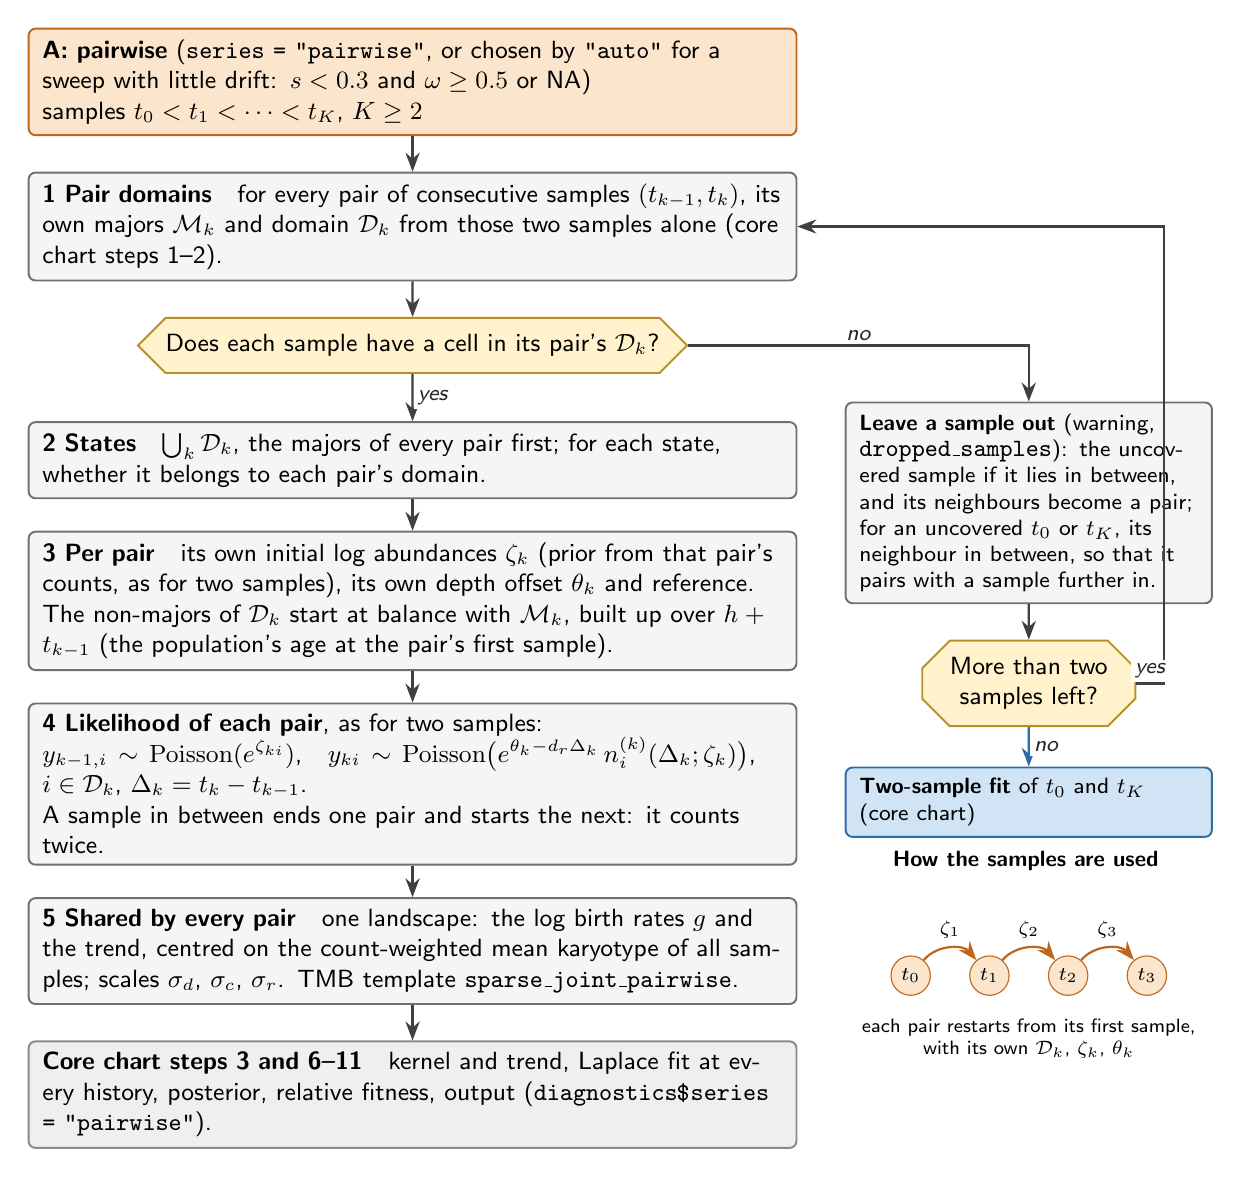
\begin{tikzpicture}

\node[box=cPair, w=9.4cm] (in) at (0,0) {%
  \textbf{A: pairwise} (\code{series = "pairwise"}, or chosen by \code{"auto"} for a sweep with little
  drift: $s<\autoshare$ and $\omega\ge\autoweight$ or NA)\\
  samples $t_0<t_1<\dots<t_K$, $K\ge2$};

\node[box, w=9.4cm, below=0.45cm of in] (pairs) {%
  \textbf{1 Pair domains}\quad for every pair of consecutive samples $(t_{k-1},t_k)$, its own majors
  $\mathcal M_k$ and domain $\mathcal D_k$ from those two samples alone (core chart steps 1--2).};
\node[dec, below=0.45cm of pairs] (cover) {Does each sample have a cell in its pair's $\mathcal D_k$?};
\draw[arr] (in) -- (pairs);
\draw[arr] (pairs) -- (cover);

% coverage loop, right-hand column
\node[box, w=4.3cm, font=\footnotesize, anchor=north west] (leave) at ($(cover.south -| pairs.east)+(0.6,-0.35)$) {%
  \textbf{Leave a sample out} (warning, \code{dropped\_samples}): the uncovered sample if it lies in
  between, and its neighbours become a pair; for an uncovered $t_0$ or $t_K$, its neighbour in between,
  so that it pairs with a sample further in.};
\node[dec, below=0.45cm of leave] (two) {More than two\\samples left?};
\node[box=cTwo, w=4.3cm, font=\footnotesize, below=0.5cm of two] (twofit) {%
  \textbf{Two-sample fit} of $t_0$ and $t_K$ (core chart)};
\draw[arr] (cover.east) -| node[lab, above, pos=0.25] {no} (leave.north);
\draw[arr] (leave) -- (two);
\draw[arr, draw=cTwoB] (two) -- node[lab, right] {no} (twofit);
\draw[arr] (two.east) -- ++(0.35,0) node[lab, above, pos=0.5] {yes} |- (pairs.east);

\node[box, w=9.4cm, below=0.6cm of cover] (states) {%
  \textbf{2 States}\quad $\bigcup_k\mathcal D_k$, the majors of every pair first; for each state,
  whether it belongs to each pair's domain.};
\draw[arr] (cover) -- node[lab, right] {yes} (states);

\node[box, w=9.4cm, below=0.4cm of states] (own) {%
  \textbf{3 Per pair}\quad its own initial log abundances $\zeta_k$ (prior from that pair's counts, as
  for two samples), its own depth offset $\theta_k$ and reference. The non-majors of $\mathcal D_k$
  start at balance with $\mathcal M_k$, built up over $h+t_{k-1}$ (the population's age at the pair's
  first sample).};
\node[box, w=9.4cm, below=0.4cm of own] (lik) {%
  \textbf{4 Likelihood of each pair}, as for two samples:\\
  $y_{k-1,i}\sim\mathrm{Poisson}(e^{\zeta_{ki}})$,\quad
  $y_{ki}\sim\mathrm{Poisson}\bigl(e^{\theta_k-d_r\Delta_k}\,n^{(k)}_i(\Delta_k;\zeta_k)\bigr)$,\quad
  $i\in\mathcal D_k$, $\Delta_k=t_k-t_{k-1}$.\\
  A sample in between ends one pair and starts the next: it counts twice.};
\node[box, w=9.4cm, below=0.4cm of lik] (shared) {%
  \textbf{5 Shared by every pair}\quad one landscape: the log birth rates $g$ and the trend, centred on
  the count-weighted mean karyotype of all samples; scales $\sigma_d$, $\sigma_c$, $\sigma_r$.
  TMB template \code{sparse\_joint\_pairwise}.};
\draw[arr] (states) -- (own);
\draw[arr] (own) -- (lik);
\draw[arr] (lik) -- (shared);

\node[box=cCore, w=9.4cm, below=0.45cm of shared] (core) {%
  \textbf{Core chart steps 3 and 6--11}\quad kernel and trend, Laplace fit at every history, posterior,
  relative fitness, output (\code{diagnostics\$series = "pairwise"}).};
\draw[arr] (shared) -- (core);

% ---- schematic --------------------------------------------------------------
\begin{scope}[shift={($(twofit.south)+(-0.5,-1.75)$)}]
  \node[font=\footnotesize\bfseries, anchor=west] at (-1.35,1.45) {How the samples are used};
  \foreach \k/\x in {0/-1.0, 1/0.0, 2/1.0, 3/2.0} {
    \node[circle, draw=cPairB, fill=cPair, minimum size=5mm, inner sep=0pt, font=\scriptsize] (s\k) at (\x,0) {$t_\k$};
  }
  \foreach \a/\b/\k in {s0/s1/1, s1/s2/2, s2/s3/3} {
    \draw[->, cPairB, line width=0.8pt] (\a) to[bend left=50] node[above, font=\scriptsize, text=black] {$\zeta_\k$} (\b);
  }
  \node[font=\scriptsize, align=center] at (0.5,-0.8) {each pair restarts from its first sample,\\
    with its own $\mathcal D_k$, $\zeta_k$, $\theta_k$};
\end{scope}

\end{tikzpicture}
\end{document}
